\documentclass[aspectratio=169,11pt]{beamer}
\usetheme{metropolis}
\usepackage{booktabs}
\usepackage{amsmath}
\usepackage{tikz}
\usepackage{appendixnumberbeamer}
\usepackage{listings}
\graphicspath{{../figures/}}

\definecolor{kal}{HTML}{EB6834}
\definecolor{rw}{HTML}{2A78D6}
\definecolor{dia}{HTML}{1BAF7A}
\setbeamercolor{alerted text}{fg=kal}
\metroset{progressbar=frametitle, numbering=fraction}

\definecolor{codebg}{HTML}{F4F4F2}
\definecolor{codecomment}{HTML}{6B6B66}
\lstdefinestyle{py}{language=Python, basicstyle=\ttfamily\scriptsize,
  keywordstyle=\color{rw}\bfseries, commentstyle=\color{codecomment},
  stringstyle=\color{dia!70!black}, showstringspaces=false,
  backgroundcolor=\color{codebg}, frame=none, xleftmargin=4pt, xrightmargin=4pt,
  aboveskip=2pt, belowskip=2pt, columns=fullflexible, keepspaces=true,
  emph={self}, emphstyle=\color{kal}}
\lstdefinestyle{term}{language={}, backgroundcolor=\color{black!85},
  basicstyle=\ttfamily\scriptsize\color{white}, frame=none, xleftmargin=4pt,
  xrightmargin=4pt, aboveskip=2pt, belowskip=2pt, columns=fullflexible, keepspaces=true}
\lstset{style=py}

\newcommand{\x}{\mathbf{x}}
\newcommand{\w}{\mathbf{w}}

\title{Correlated Uncertainty, Not Drift}
\subtitle{What a Kalman-filter learner explains about retrospective revaluation that Rescorla--Wagner cannot}
\author{Solanki Viraj Rajeshbhai \quad 24110348}
\institute{CG-501 Computation and Cognition --- End-Term Presentation}
\date{November 2026}

\begin{document}

\maketitle

%---------------------------------------------------------------
\begin{frame}{What is this project about?}
\textbf{How do we learn what causes what?}
\vspace{0.5em}
\begin{columns}[T]
\column{0.55\textwidth}
\small
\textbf{An everyday example}
\begin{enumerate}
\item You eat \textbf{shrimp and peanuts} together and get a rash.\\
\emph{Which food caused it? You can't tell yet.}
\item Later you eat \textbf{peanuts alone} and get the same rash.
\item Now you think: \emph{``the peanuts did it, the shrimp is probably fine.''}
\end{enumerate}
\vspace{0.3em}
You changed your mind about the shrimp \alert{without eating shrimp again}.
Psychologists call this \alert{backward blocking}.
\column{0.42\textwidth}
\small
\begin{block}{What I do in this project}
I build \textbf{computer models} of a learner, run classic learning
experiments \textbf{in simulation}, and check:
\begin{itemize}
\item which model can learn like this,
\item and \textbf{which part} of the model makes it possible.
\end{itemize}
\end{block}
\end{columns}
\end{frame}

%---------------------------------------------------------------
\begin{frame}{The few terms you need}
\begin{columns}[T]
\column{0.46\textwidth}
\begin{itemize}\small
\item \textbf{Cue} (A, B, C): something the learner notices, e.g.\ a food, a light, a sound.
\item \textbf{Outcome}: what follows the cue, e.g.\ a rash or a reward.
\item \textbf{Trial}: one experience, e.g.\ one meal.
\item \textbf{Weight} $w$: how strongly the learner believes a cue predicts the outcome, from 0 (not at all) to 1 (always).
\end{itemize}
\column{0.5\textwidth}
\textbf{Notation on the slides}
\vspace{0.3em}

\small
\begin{tabular}{@{}ll@{}}
\toprule
AB$+$ & A and B together, outcome follows\\
B$+$ & B alone, outcome follows\\
A$-$ & A alone, no outcome\\
AB$+\to$B$+$ & first AB$+$ trials, then B$+$ trials\\
\bottomrule
\end{tabular}

\vspace{0.6em}
\small Shrimp example: A = shrimp, B = peanuts.\\
AB$+$ then B$+$ $\Rightarrow$ $w_A$ should go \alert{down}.
\end{columns}
\end{frame}

%---------------------------------------------------------------
\begin{frame}{The question}
\begin{itemize}
\item The classic model of this kind of learning is the \textcolor{rw}{\textbf{Rescorla--Wagner (RW)}} model (1972).
\item It has a blind spot: a cue that is \alert{not present} on a trial can never change its weight.
So RW can never change its mind about the shrimp.
\item A \textcolor{kal}{\textbf{Kalman-filter learner}} is a Bayesian learner: it keeps track not only of its beliefs,
but also of \textbf{how sure} it is about them.
\end{itemize}
\vspace{0.4em}
\begin{block}{Research question}
Can a Kalman-filter learner explain these ``change your mind about an absent cue'' effects,
which RW cannot? And \textbf{which component} of the Kalman filter is responsible?
\end{block}
\vspace{0.3em}
\small\textbf{What I did:} implement 4 models $\to$ check the code is correct $\to$ simulate 6 classic
experiments $\to$ remove parts of the model one at a time to see what breaks.
\end{frame}

%---------------------------------------------------------------
\begin{frame}{Background: four classic effects}
\centering
\small
\begin{tabular}{llll}
\toprule
Effect & Phase 1 & Phase 2 & What happens\\
\midrule
Forward blocking & A$+$ & AB$+$ & A already explains the outcome, so B learns little\\
Overshadowing & AB$+$ & & A and B share the credit\\
\alert{Backward blocking} & AB$+$ & B$+$ & A \emph{loses} value, although A is absent\\
\alert{Unovershadowing} & AB$+$ & A$-$ & B \emph{gains} value, although B is absent\\
\bottomrule
\end{tabular}
\vspace{0.8em}
\begin{itemize}\small
\item The first two: the cue is present when it changes. RW explains both.
\item The last two (\textbf{retrospective revaluation}): the cue is \emph{absent} when it changes.
Shown in people (Shanks, 1985) and in animals, though less reliably (Matzel et al., 1985; Miller \& Matute, 1996).
\end{itemize}
\end{frame}

%---------------------------------------------------------------
\begin{frame}{Background: Rescorla--Wagner and its successors}
\textbf{RW in plain words:} surprise $=$ what happened $-$ what I expected.
Every \emph{present} cue moves its weight by a share of the surprise.
\[
\delta = r - \textstyle\sum_j x_j w_j, \qquad w_i \leftarrow w_i + \alpha\, x_i\,\delta
\qquad (x_i = 1 \text{ if cue } i \text{ is present, else } 0)
\]
\begin{itemize}\small
\item Present cues share one surprise, so they compete: blocking and overshadowing.
\item Absent cue: $x_i = 0$, so its change is 0. \alert{No backward blocking, ever.}
\end{itemize}
\vspace{0.2em}
\textbf{Earlier work: learning as Kalman filtering}
\begin{itemize}\footnotesize
\item Sutton (1992); Dayan, Kakade \& Montague (2000): learning rates follow uncertainty, but each cue's uncertainty is tracked \emph{separately}.
\item Dayan \& Kakade (2001): tracking how uncertainties about cues are \emph{linked} gives backward blocking.
\item Van Hamme \& Wasserman (1994): a non-Bayesian fix, where absent cues are ``remembered''.
\end{itemize}
\end{frame}

%---------------------------------------------------------------
\begin{frame}{Hypotheses}
\begin{description}[H2]
\item[H1] The Kalman learner \textbf{can} change its mind about absent cues (backward blocking,
unovershadowing); RW \textbf{cannot}. Both show forward blocking and overshadowing.
\item[H2] The key ingredient is the \textbf{link between cues} (the cross-cue covariance).
Removing it should remove these effects, but keep forward blocking.
\item[H3] A learner that expects the world to change (more drift, $\tau^2$) stays more uncertain,
so it should learn faster and show \textbf{stronger} backward blocking.
\end{description}
\end{frame}

%---------------------------------------------------------------
\begin{frame}{Methods: the Kalman learner}
\textbf{In plain words:} like RW, but the learner also keeps a measure of how unsure it is
about each weight, and \alert{how its uncertainties about different cues are linked}.
Unsure weights learn faster.
\vspace{0.3em}
\begin{columns}[T]
\column{0.5\textwidth}
\footnotesize
\textbf{It assumes:} weights drift a little each trial (variance $\tau^2$) and outcomes are noisy (variance $\sigma^2$).
\vspace{0.4em}

\textbf{It keeps:} a mean $\hat\w$ (its best guess) and a covariance matrix $\Sigma$ (its uncertainty).
The off-diagonal entry $\Sigma_{AB}$ is the link between A and B.
\column{0.48\textwidth}
\footnotesize
\textbf{Every trial:}
\begin{align*}
\Sigma^- &= \Sigma + \tau^2 I && \text{unsure-ness grows}\\
\mathbf k &= \frac{\Sigma^-\x}{\x^\top\Sigma^-\x + \sigma^2} && \text{learning rate per cue}\\
\hat\w &\leftarrow \hat\w + \mathbf k\,\delta && \text{like RW}\\
\Sigma &\leftarrow \Sigma^- - \mathbf k\,(\Sigma^-\x)^\top && \text{unsure-ness shrinks}
\end{align*}
\end{columns}
\vspace{0.3em}
\small\alert{Key:} an absent cue A gets learning rate $k_A \propto \Sigma_{AB}$. If A and B are linked, A can learn even when it is absent.
\end{frame}

%---------------------------------------------------------------
\begin{frame}{Methods: why A and B become linked}
\begin{columns}[c]
\column{0.55\textwidth}
\begin{itemize}
\item AB$+$ trials only tell the learner that \emph{together} they predict the outcome: $w_A + w_B \approx 1$.
\item 0.5 and 0.5, or 0.9 and 0.1, or 0.1 and 0.9: all fit equally well.
\item So it is sure about the \emph{sum} but not the \emph{split}: if A is high, B must be low. That is a \alert{negative link}, $\Sigma_{AB} < 0$.
\item Then B$+$: B alone explains the outcome, so A must be low. A is \emph{explained away}.
\end{itemize}
\column{0.42\textwidth}
\centering
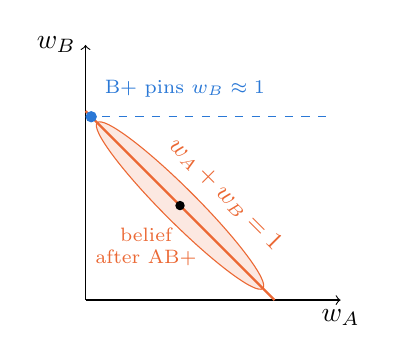
\begin{tikzpicture}[scale=2.4]
\draw[->] (0,0) -- (1.35,0) node[below] {$w_A$};
\draw[->] (0,0) -- (0,1.35) node[left] {$w_B$};
\draw[thick, kal] (0,1) -- (1,0);
\node[kal, font=\small, rotate=-45] at (0.74,0.56) {$w_A+w_B=1$};
\node[kal, font=\scriptsize, align=center] at (0.32,0.28) {belief\\after AB$+$};
\draw[rotate around={-45:(0.5,0.5)}, kal, fill=kal, fill opacity=0.15] (0.5,0.5) ellipse (0.62 and 0.09);
\fill (0.5,0.5) circle (0.025);
\draw[dashed, rw] (0,0.97) -- (1.3,0.97);
\node[rw, font=\scriptsize, anchor=west] at (0.05,1.12) {B$+$ pins $w_B\approx1$};
\fill[rw] (0.03,0.97) circle (0.03);
\end{tikzpicture}
\end{columns}
\end{frame}

%---------------------------------------------------------------
\begin{frame}{Methods: models, design, validation}
\begin{columns}[t]
\column{0.5\textwidth}
\textbf{4 models compared}
\begin{itemize}\small
\item \textcolor{rw}{RW}: the classic model
\item \textcolor{kal}{Kalman, full}: with links between cues
\item \textcolor{dia}{Kalman, diagonal}: links deleted (the ``ablation'')
\item RW + within-compound: the non-Bayesian alternative
\end{itemize}
\textbf{Experiments}
\begin{itemize}\small
\item 6 classic designs, each with a matched control
\item Sweep: 100 combinations of $\tau^2$ and $\sigma^2$
\item Noisy outcomes, 20 random seeds
\end{itemize}
\column{0.5\textwidth}
\textbf{Checking the code first (10 tests, all pass)}
\begin{itemize}\small
\item RW matches its exact formula
\item Kalman with no drift $=$ textbook Bayesian regression, after \emph{every} trial, to $10^{-9}$
\end{itemize}
\textbf{Data}
\begin{itemize}\small
\item All simulated, no external dataset
\item One command regenerates everything
\end{itemize}
\end{columns}
\end{frame}

%---------------------------------------------------------------
\begin{frame}{Result 1: my code reproduces a published simulation}
\centering
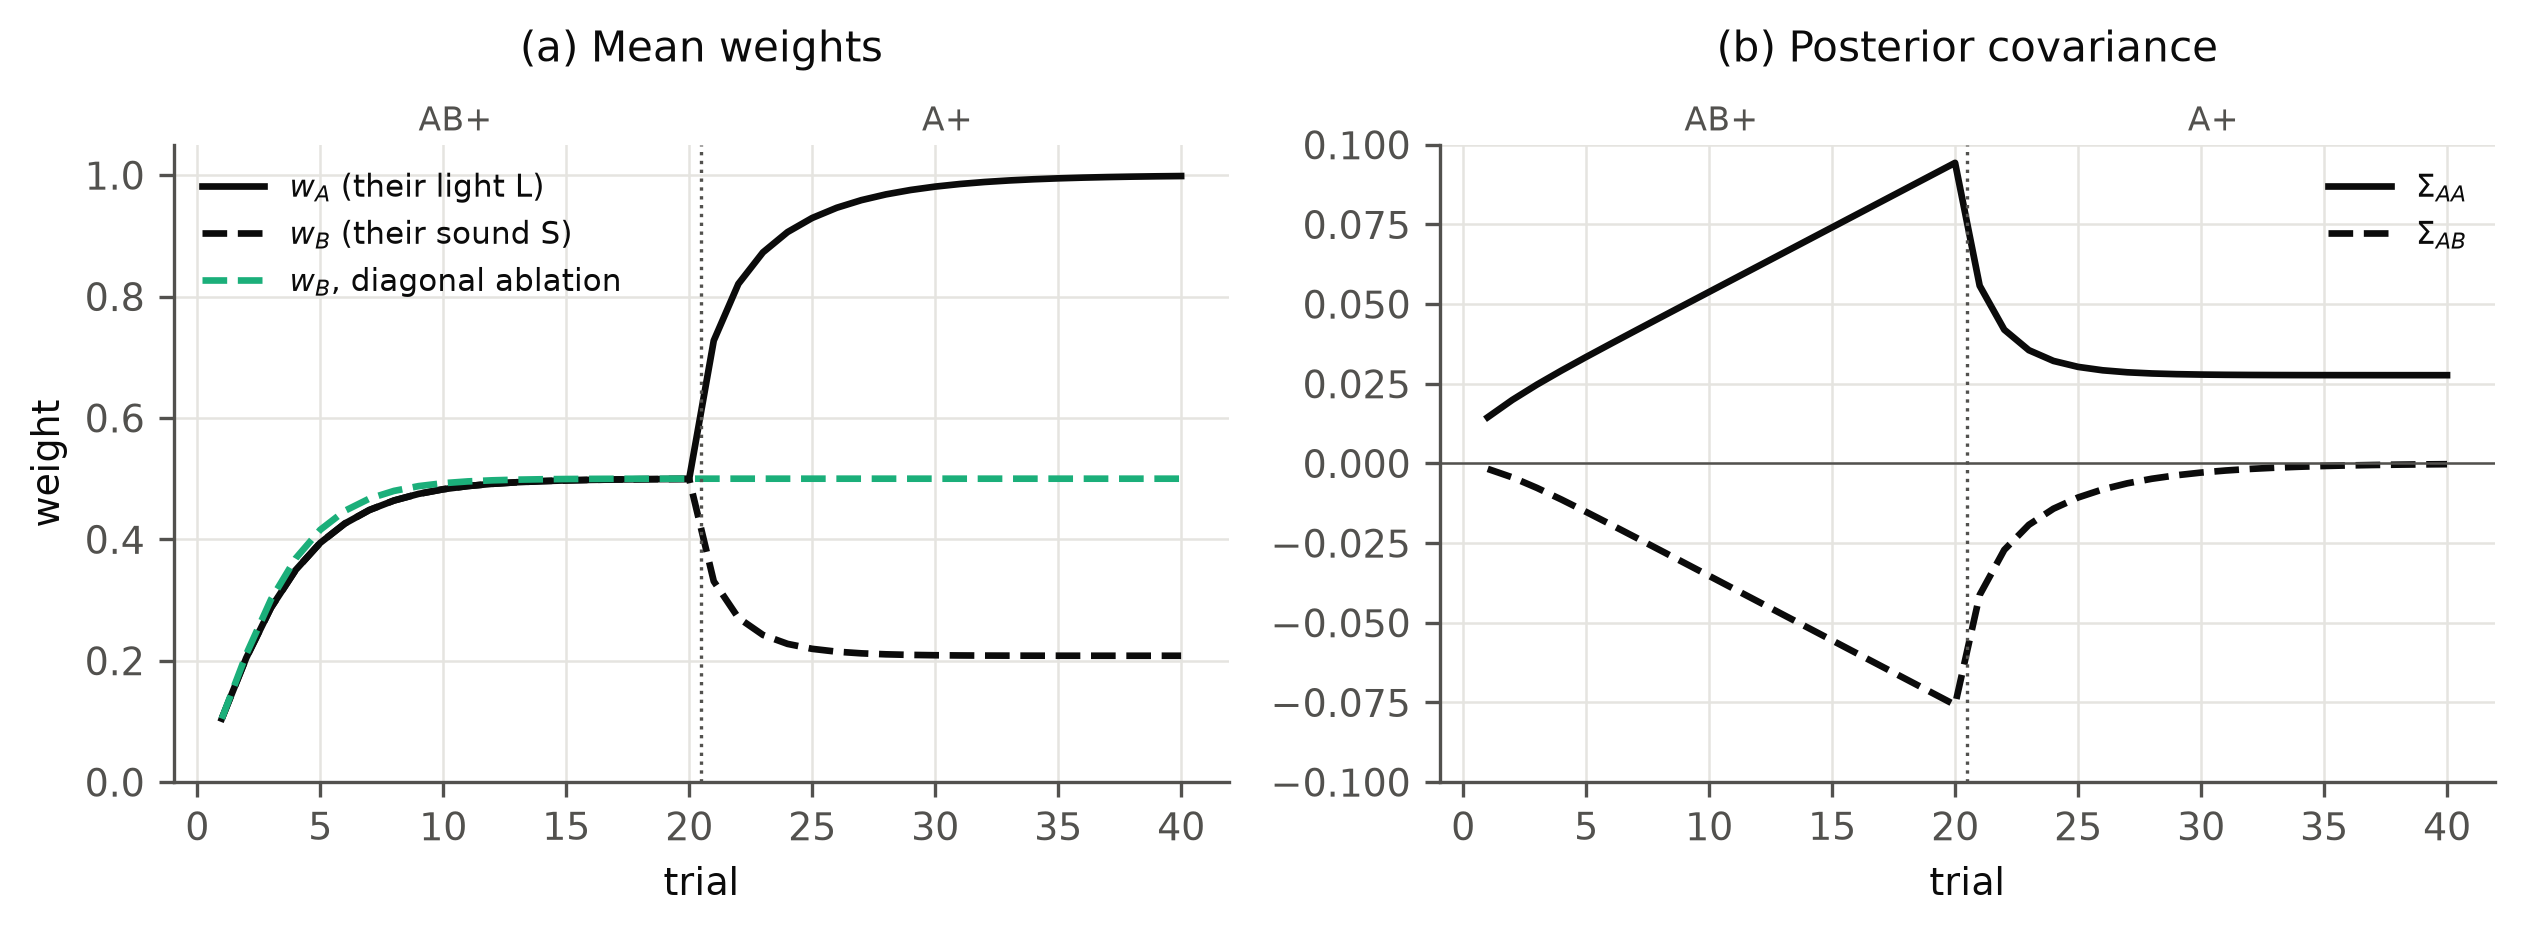
\includegraphics[width=0.8\textwidth]{fig7_dk2001_replication.png}\\[0.2em]
\small Dayan \& Kakade (2001), with their parameters (prior assumed).
After AB$+$ then A$+$, B is explained away: it falls to 0.21.
The link $\Sigma_{AB}$ turns negative ($-0.076$). Diagonal model: no change.
\end{frame}

%---------------------------------------------------------------
\begin{frame}{Result 2: only the full Kalman learner changes its mind about absent cues (H1)}
\centering
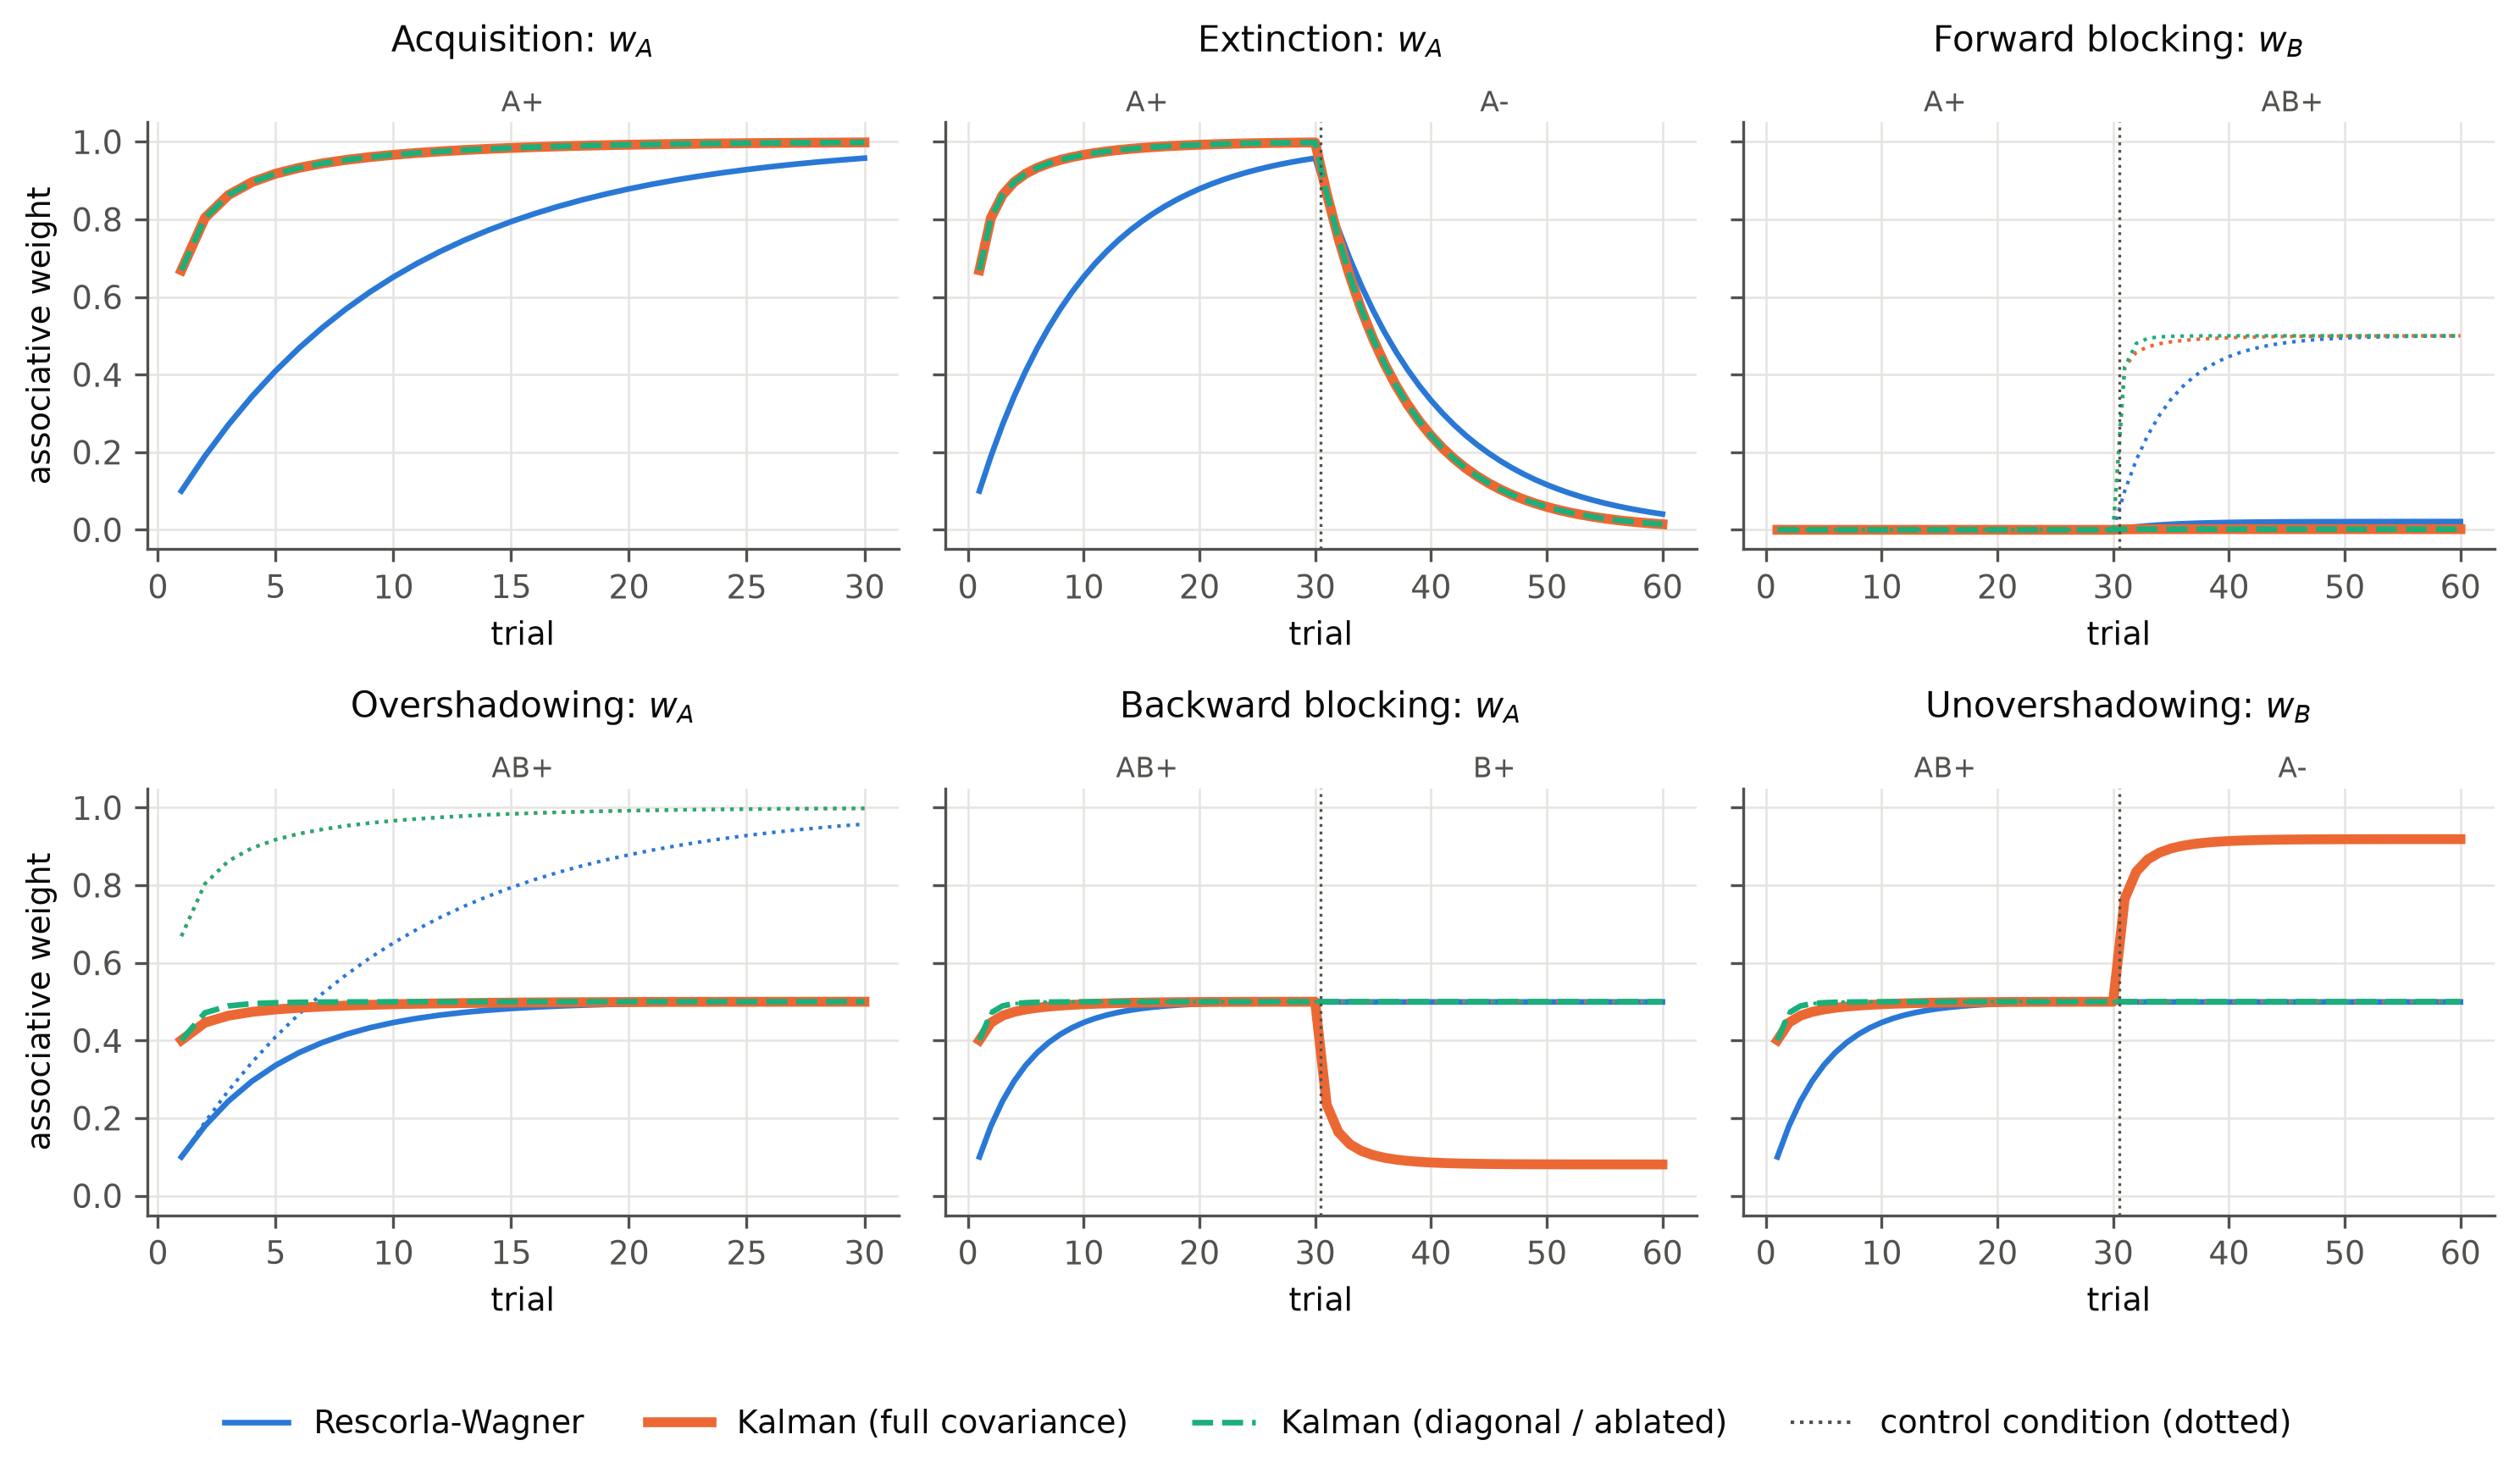
\includegraphics[width=0.72\textwidth]{fig1_replication.png}\\[0.1em]
\footnotesize Each panel is one experiment; lines show the weight of the cue that matters.
All models agree on the top row and on overshadowing. Only \textcolor{kal}{orange} moves in backward blocking and unovershadowing.
\end{frame}

%---------------------------------------------------------------
\begin{frame}{Result 2: how big are the effects?}
\centering
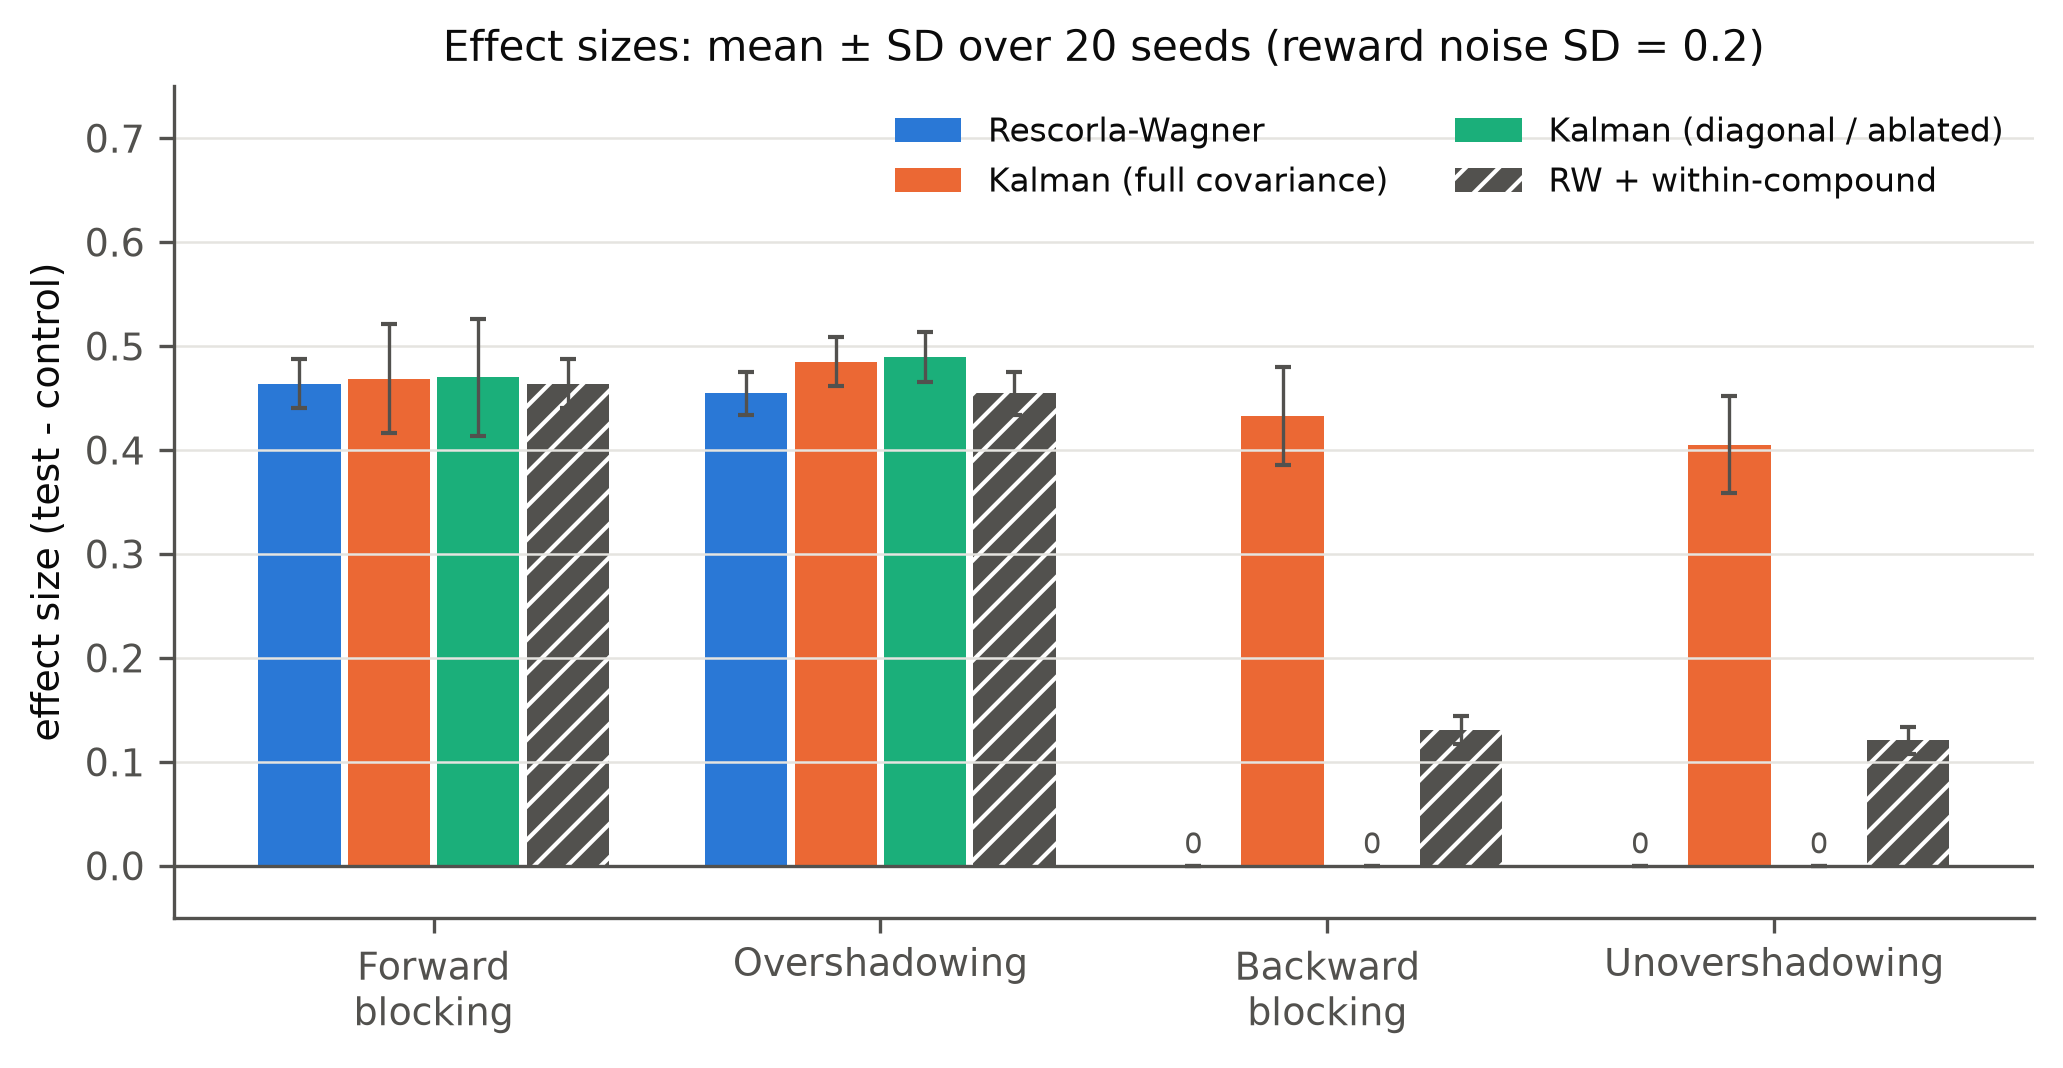
\includegraphics[width=0.68\textwidth]{fig2_effect_sizes.png}\\[0.2em]
\small Effect = test minus control (0 = no effect, 0.5 = very large).
With noisy outcomes, Kalman: backward blocking $0.433\pm0.047$, unovershadowing $0.405\pm0.047$, in 20 of 20 runs.
RW and diagonal: exactly 0.
\end{frame}

%---------------------------------------------------------------
\begin{frame}{Result 3: how it happens, trial by trial}
\centering
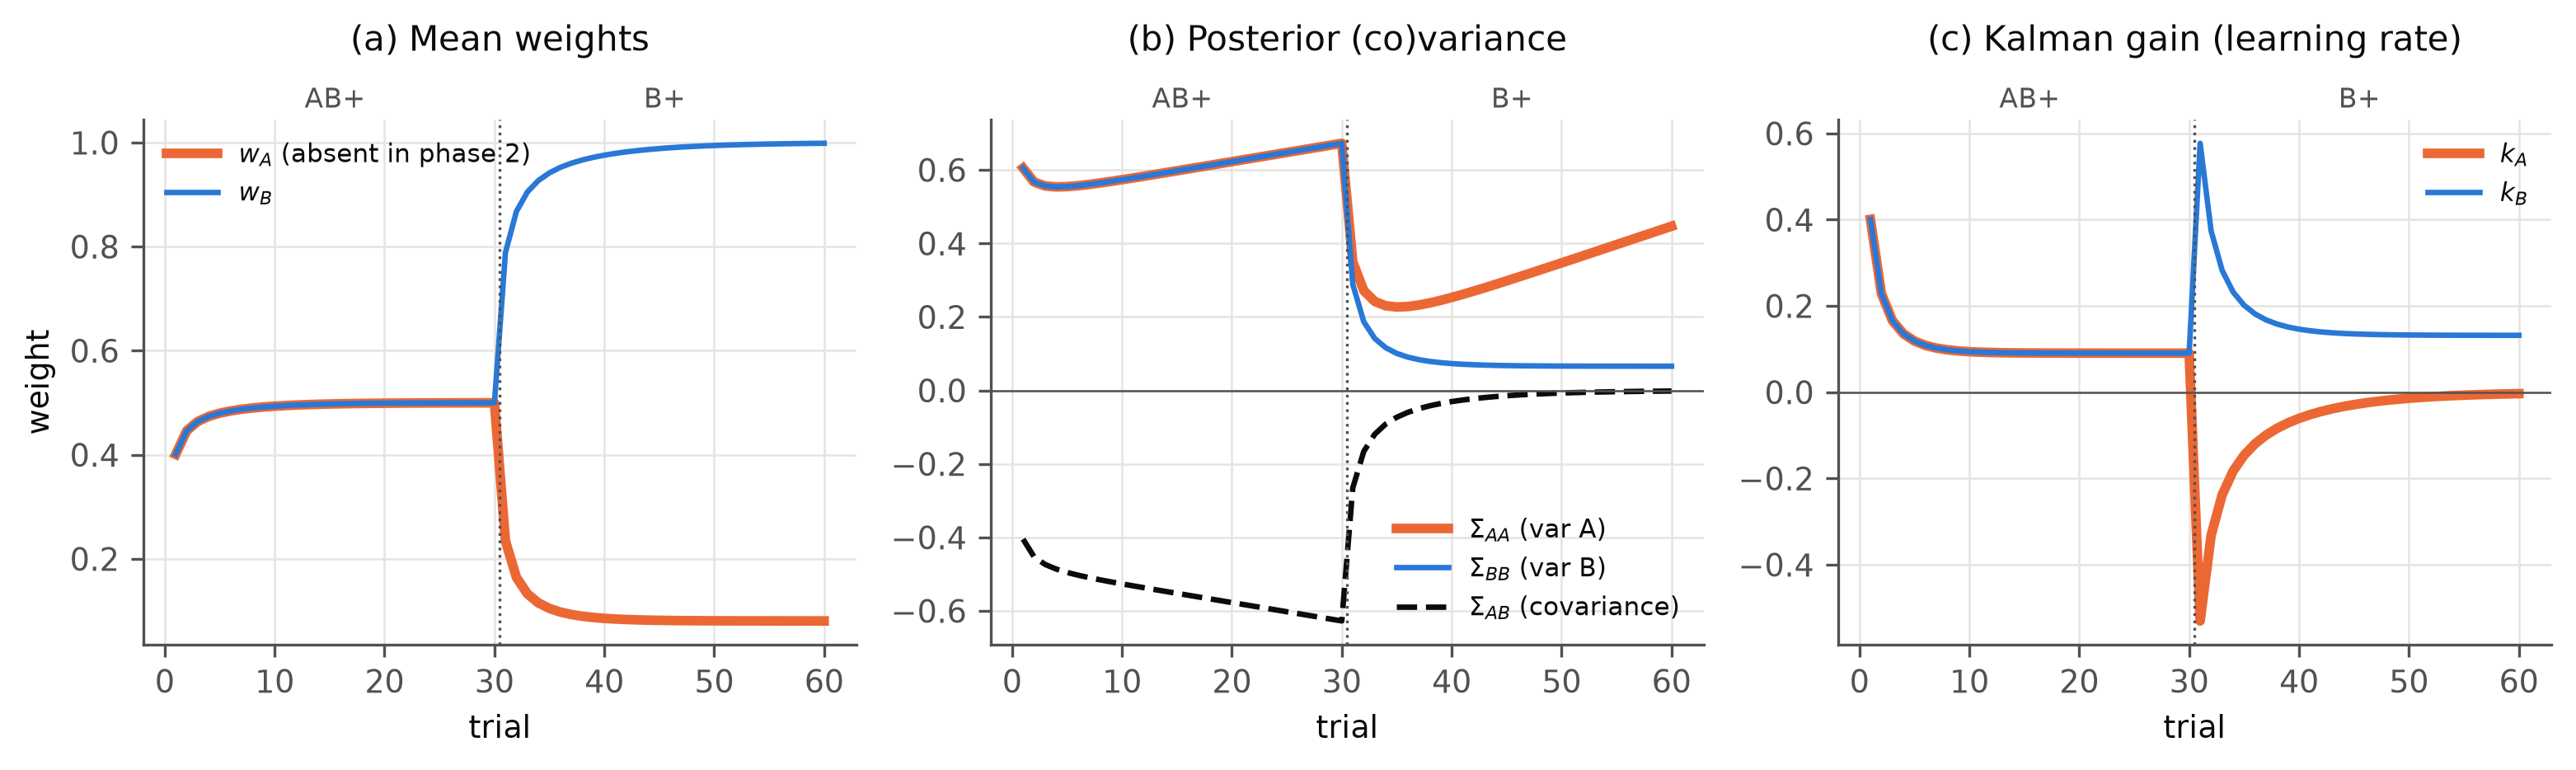
\includegraphics[width=0.95\textwidth]{fig3_kalman_mechanism.png}\\[0.3em]
\small After AB$+$, the link is $\Sigma_{AB} = -0.627$. On the first B$+$ trial, A's learning rate is
$k_A = -0.627/1.183 = -0.53$, and the surprise is $\delta = 0.5$.\\
So $w_A$ drops from $0.50$ to $0.24$ in one trial, \alert{although A is not present}.
\end{frame}

%---------------------------------------------------------------
\begin{frame}{Result 4: drift is \emph{not} needed (H3 rejected)}
\centering
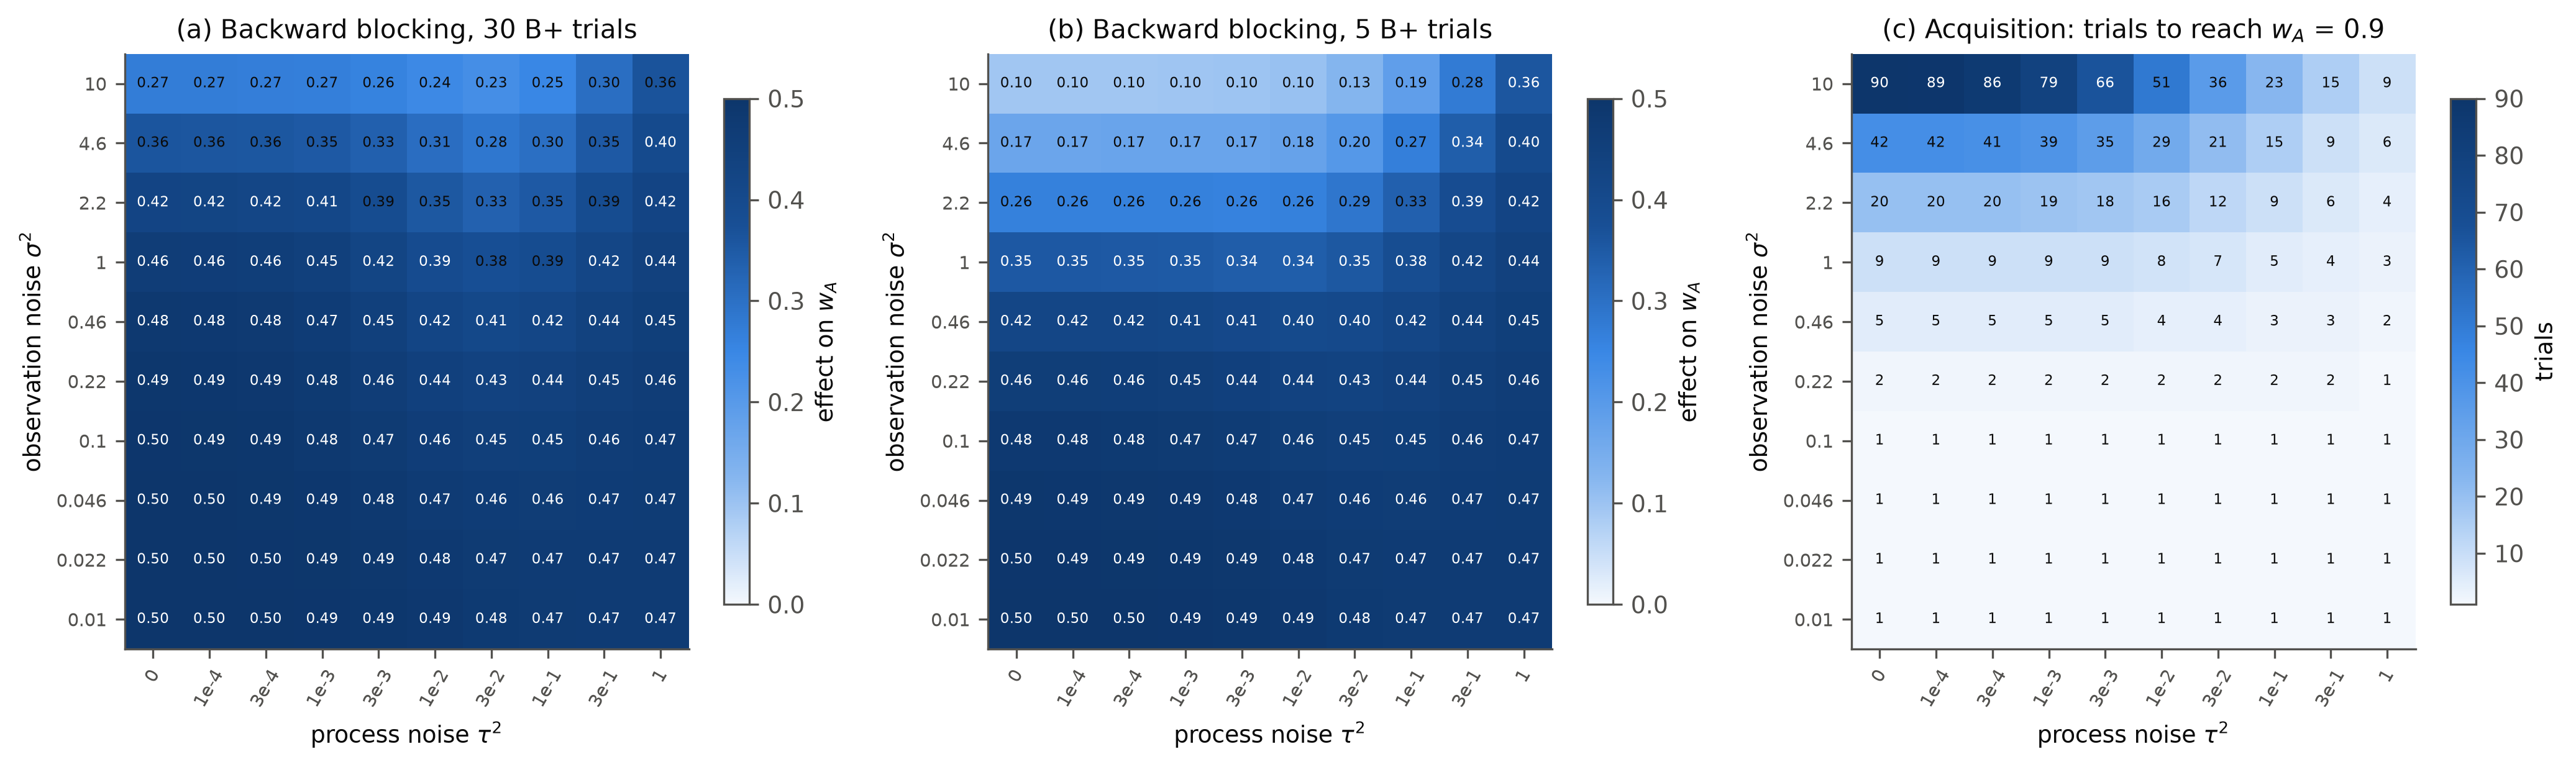
\includegraphics[width=0.98\textwidth]{fig4_noise_sweep.png}\\[0.2em]
\small Backward blocking appears at all 100 settings, \textbf{even with zero drift} ($\tau^2 = 0$: 0.27 to 0.50).
The link comes from training A and B together, not from drift.
More outcome noise slows it (b). Drift mostly speeds up ordinary learning (c).
\end{frame}

%---------------------------------------------------------------
\begin{frame}{Result 5: remove the link, and the effect disappears (H2)}
\centering
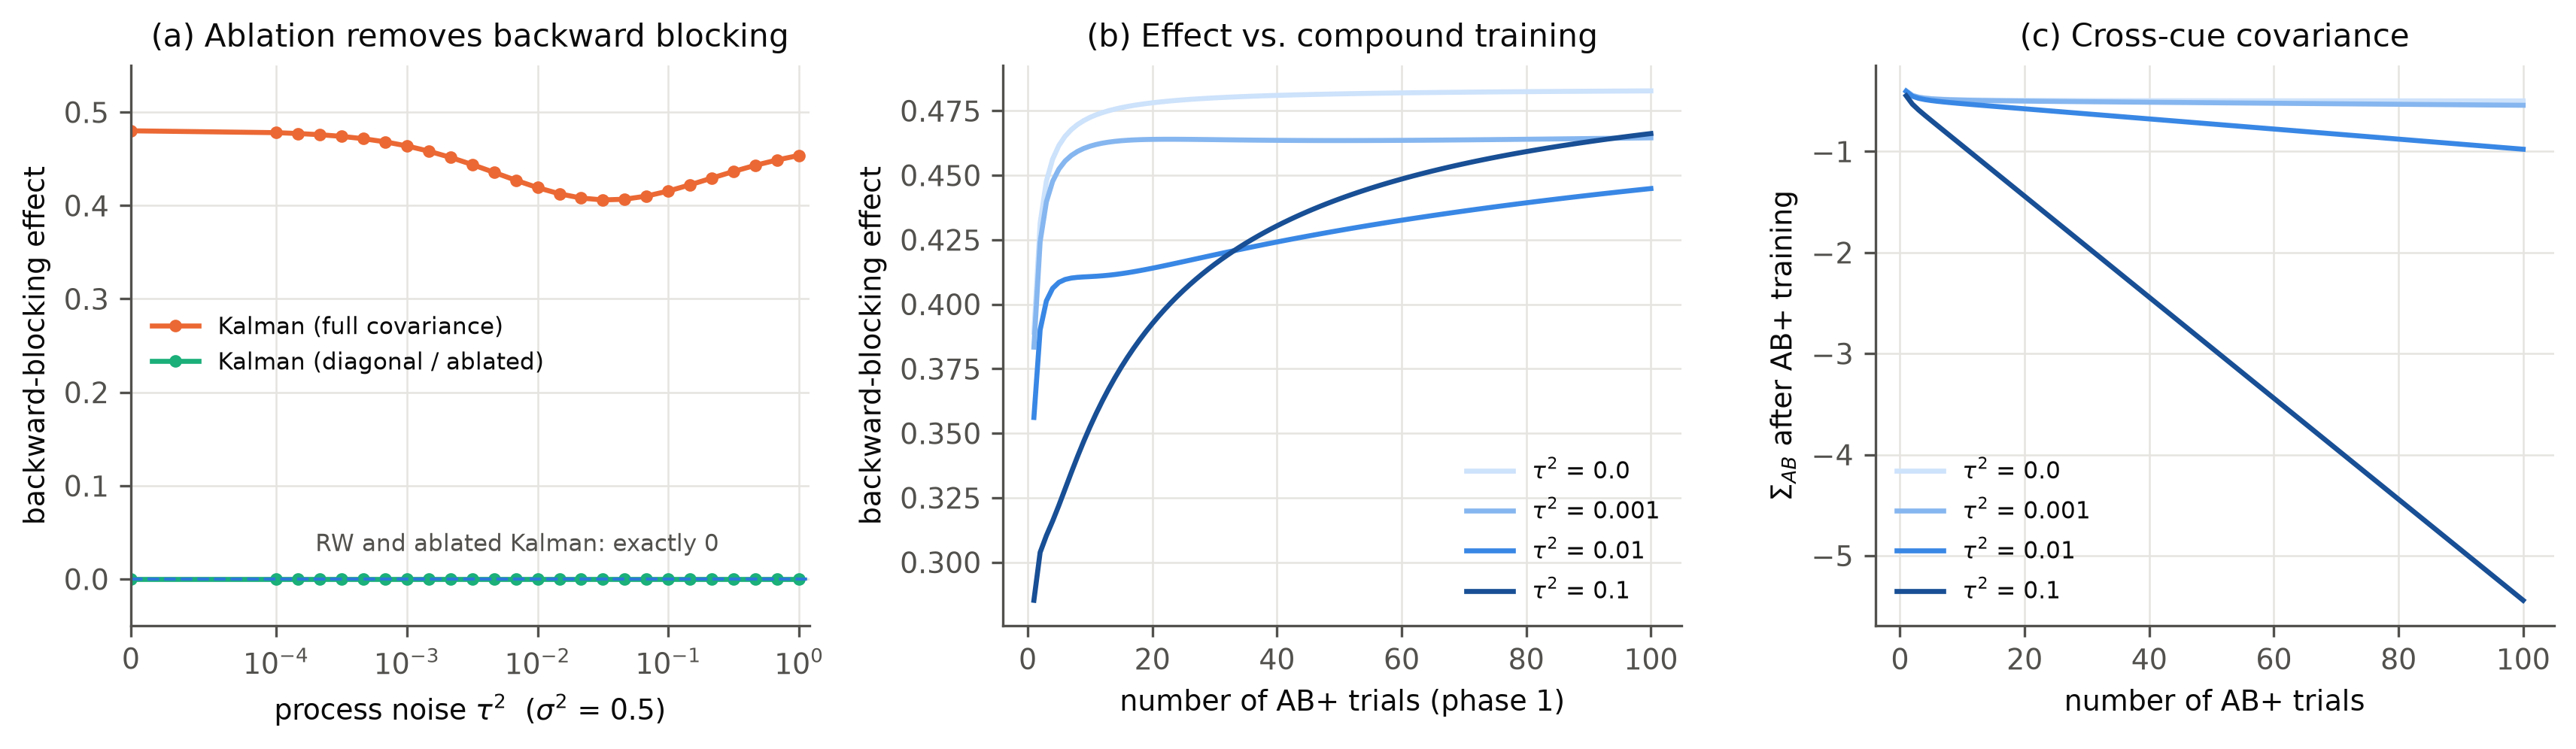
\includegraphics[width=0.98\textwidth]{fig5_ablation.png}\\[0.2em]
\small (a) Without the link, backward blocking is 0 everywhere, but forward blocking survives (0.31 to 0.50).
So forward blocking comes from the shared surprise, and changing your mind comes from the link.
(c) With drift, the link keeps growing during AB$+$ training.
\end{frame}

%---------------------------------------------------------------
\begin{frame}{Result 6: another model can do it too}
\begin{columns}[c]
\column{0.52\textwidth}
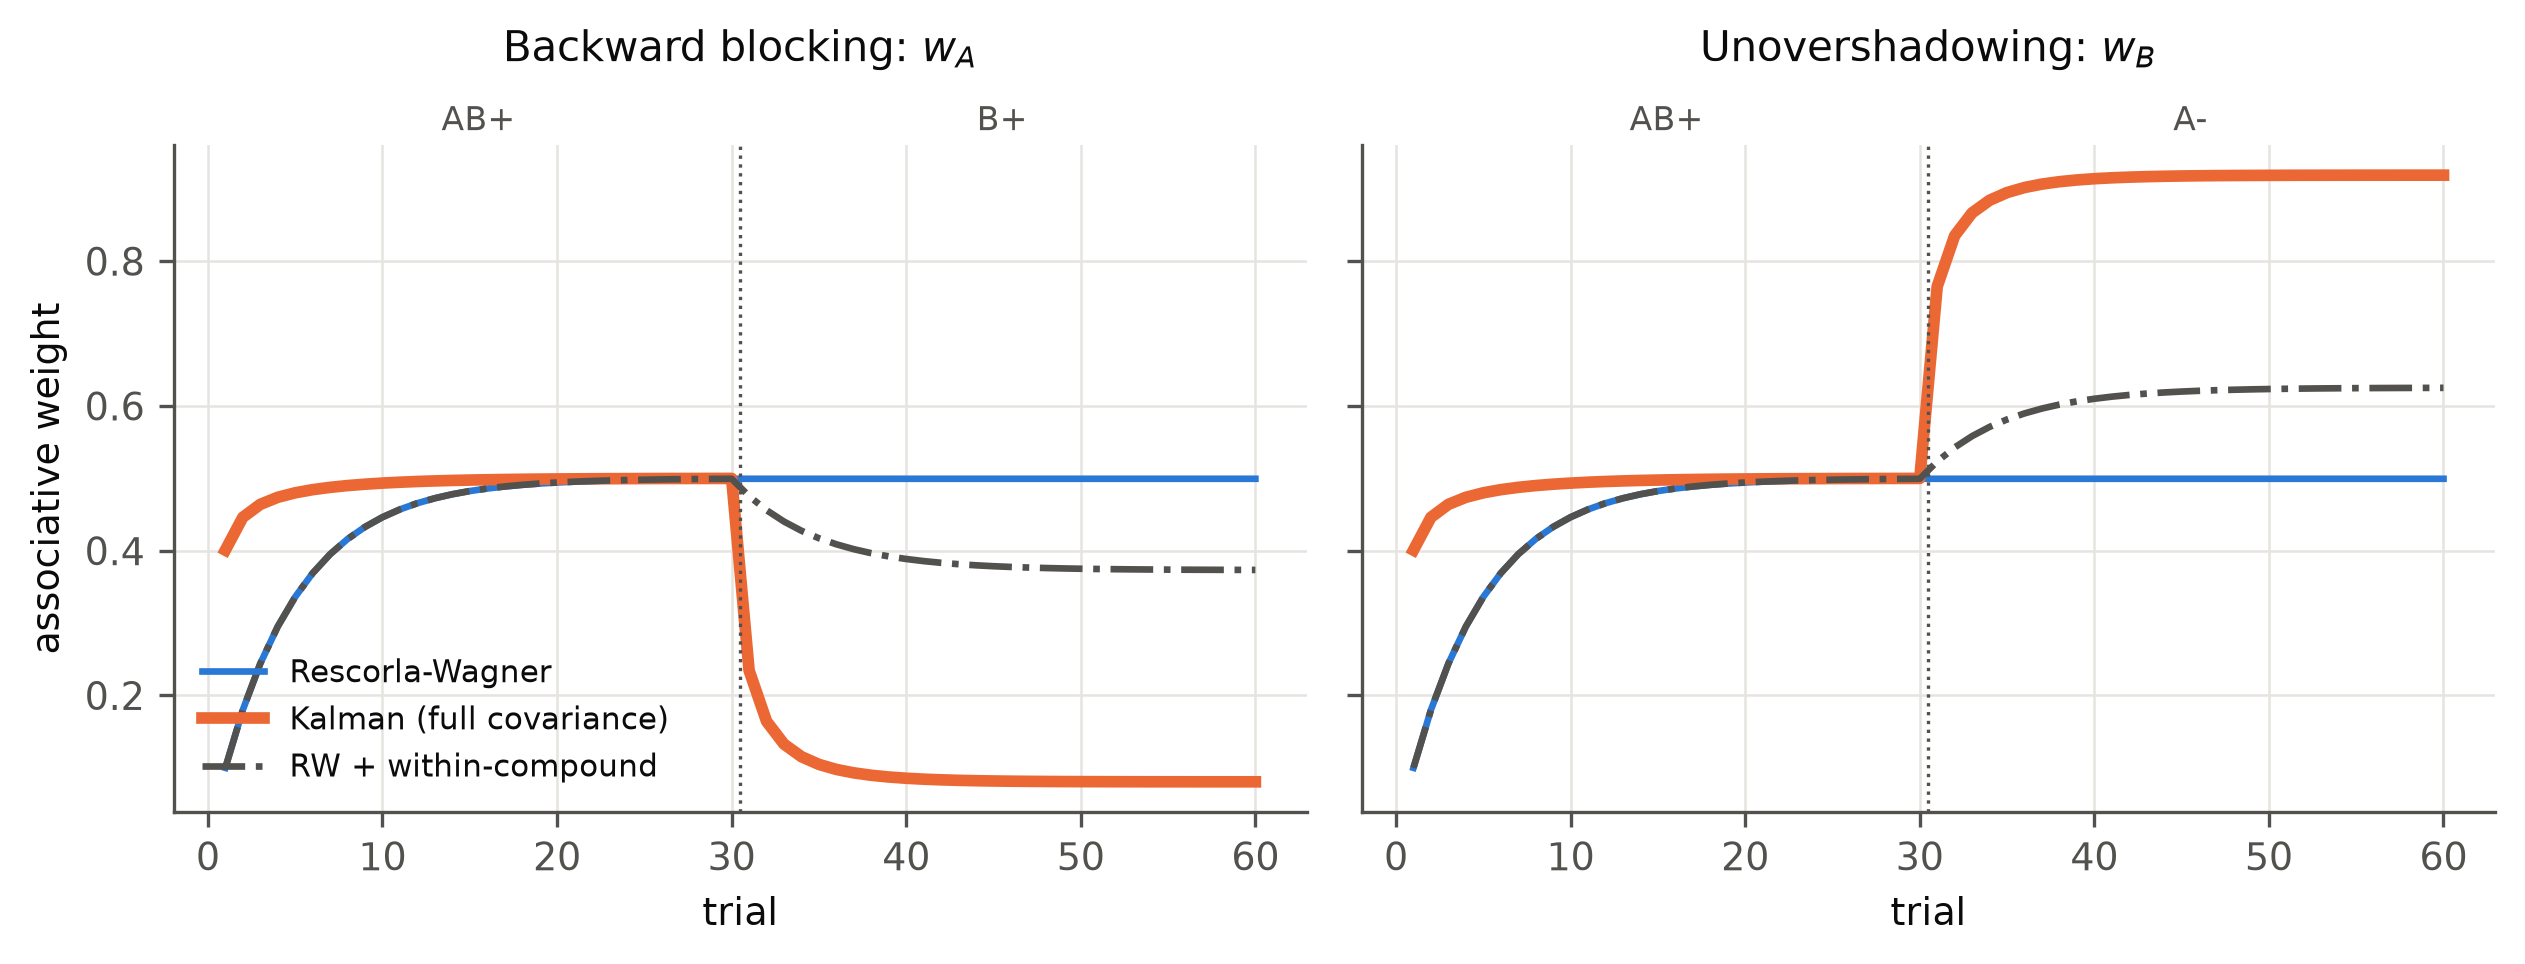
\includegraphics[width=\textwidth]{fig6_alternative_model.png}
\column{0.46\textwidth}
\footnotesize
RW + within-compound (absent cues are ``remembered''): backward blocking $0.13$, unovershadowing $0.12$.\\[0.6em]
\textbf{How to tell them apart: trial order}\\
Same trials, two orders; final $w_B$:\\[0.3em]
\setlength{\tabcolsep}{3pt}\begin{tabular}{lcc}
\toprule
 & A$+\!\to$AB$+$ & AB$+\!\to$A$+$\\
\midrule
Kalman $\tau^2{=}0$ & 0.016 & 0.016\\
Kalman $\tau^2{=}0.01$ & 0.002 & 0.081\\
Within-compound & 0.021 & 0.373\\
\bottomrule
\end{tabular}\\[0.4em]
Order matters little for Kalman, a lot for the alternative.
\end{columns}
\end{frame}

%---------------------------------------------------------------
\begin{frame}{Discussion: what this means}
\begin{itemize}
\item \textbf{Explains:} the Kalman learner changes its mind about absent cues because it tracks
\alert{how its uncertainties about cues are linked}, not just because its learning rates follow uncertainty.
This supports Dayan \& Kakade's point about Sutton's simplified version.
\item \textbf{Where it fails:}
\begin{itemize}\small
\item It predicts backward blocking almost as strong as forward blocking (0.42 vs 0.50);
in animals it is much weaker (Miller \& Matute, 1996).
\item With drift, the link grows without limit.
\item Forgetting is complete: no spontaneous recovery after extinction.
\end{itemize}
\item \textbf{Alternative explanation:} remembered absent cues (Van Hamme \& Wasserman, 1994;
Wagner's SOP) give the same effects, but predict a much stronger order effect.
\end{itemize}
\end{frame}

%---------------------------------------------------------------
\begin{frame}{Limitations and future directions}
\textbf{Limitations}
\begin{itemize}\small
\item Simulated data only: no model was fitted to real behaviour.
\item The replication of Dayan \& Kakade is by eye; their prior had to be assumed.
\item Parameters were chosen by hand; the within-compound model is simplified.
\end{itemize}
\textbf{Future directions}
\begin{itemize}\small
\item Fit both models to real data from human cause-and-effect learning experiments.
\item Test the trial-order prediction, which separates the two explanations.
\item Compare with latent-cause models (Gershman, 2015).
\end{itemize}
\end{frame}

%===============================================================
\section{How the code works}

%---------------------------------------------------------------
\begin{frame}[fragile]{Code: the repository and how to reproduce it}
\begin{columns}[T]
\begin{column}{0.4\textwidth}
\small
\begin{tabular}{@{}ll@{}}
\texttt{models.py} & the four learners\\
\texttt{schedules.py} & experiment designs\\
\texttt{experiments.py} & all simulations\\
\texttt{make\_figures.py} & the 7 figures\\
\texttt{tests.py} & 10 validation tests\\
\texttt{results/} & every number\\
\texttt{report/}, \texttt{slides/} & report and slides\\
\end{tabular}

\vspace{0.8em}
\begin{itemize}\footnotesize
\item Only NumPy and Matplotlib.
\item Fixed random seeds: every run gives identical output.
\end{itemize}
\end{column}
\begin{column}{0.58\textwidth}
\begin{lstlisting}[style=term]
$ python tests.py
PASS  test_kalman_zero_process_noise_matches_ridge_...
PASS  test_rw_absent_cue_never_changes
  ...
10/10 tests passed

$ python make_figures.py
saved figures/fig1_replication.png
  ...
saved figures/fig7_dk2001_replication.png
All figures in ./figures,
numbers in ./results/summary.md
(takes about 8 seconds)
\end{lstlisting}
\end{column}
\end{columns}
\end{frame}

%---------------------------------------------------------------
\begin{frame}[fragile]{Code: \texttt{models.py}, Rescorla--Wagner}
\begin{lstlisting}
class RescorlaWagner:
    def predict(self, x):
        # predicted reward = sum of the weights of the cues that are present
        return float(np.dot(x, self.w))

    def update(self, x, r):
        # learn from one trial, return the prediction error
        x = np.asarray(x, dtype=float)
        delta = r - self.predict(x)               # how surprised were we?
        self.w = self.w + self.alpha * x * delta  # move present cues toward r
        return delta
\end{lstlisting}
\vspace{0.6em}
\begin{itemize}
\item One line of learning: $w_i \leftarrow w_i + \alpha\,x_i\,\delta$.
\item An absent cue has $x_i = 0$, so its weight \alert{never changes}. That is the blind spot.
\end{itemize}
\end{frame}

%---------------------------------------------------------------
\begin{frame}[fragile]{Code: \texttt{models.py}, the Kalman learner}
\begin{columns}[T]
\begin{column}{0.6\textwidth}
\begin{lstlisting}
def update(self, x, r):
    # (1) drift: uncertainty grows
    S_pred = self.S + self.tau2 * np.eye(self.n)
    # (2) Kalman gain
    Sx = S_pred @ x
    total_var = x @ Sx + self.sigma2
    k = Sx / total_var
    # (3) mean update, like RW with rate k
    delta = r - self.predict(x)
    self.w = self.w + k * delta
    # (4) uncertainty shrinks
    S_new = S_pred - np.outer(k, Sx)
    S_new = 0.5 * (S_new + S_new.T)  # keep symmetric
    if self.diagonal:                # the ABLATION
        S_new = np.diag(np.diag(S_new))
    self.S = S_new
    return delta
\end{lstlisting}
\end{column}
\begin{column}{0.38\textwidth}
\small
\begin{enumerate}
\item $\boldsymbol\Sigma^- = \boldsymbol\Sigma + \tau^2 \mathbf I$
\item $\mathbf k = \dfrac{\boldsymbol\Sigma^-\x}{\x^\top\boldsymbol\Sigma^-\x + \sigma^2}$
\item $\w \leftarrow \w + \mathbf k\,\delta$
\item $\boldsymbol\Sigma \leftarrow \boldsymbol\Sigma^- - \mathbf k(\boldsymbol\Sigma^-\x)^\top$
\end{enumerate}
\vspace{0.4em}
\footnotesize
\texttt{sigma2}: reward noise\\
\texttt{tau2}: drift\\
\texttt{diagonal=True}: delete the cross-cue covariance
\end{column}
\end{columns}
\end{frame}

%---------------------------------------------------------------
\begin{frame}{Code: one backward-blocking trial, by hand}
After 30 AB$+$ trials (default parameters), on the first B$+$ trial:
\vspace{0.5em}
\begin{columns}[T]
\begin{column}{0.48\textwidth}
\centering
\begin{tabular}{lr}
\toprule
Quantity & Value\\
\midrule
$\Sigma^-_{AB}$ & $-0.627$\\
$\Sigma^-_{BB}$ & $0.683$\\
total variance $\Sigma^-_{BB} + \sigma^2$ & $1.183$\\
prediction error $\delta$ & $0.5$\\
\bottomrule
\end{tabular}
\end{column}
\begin{column}{0.5\textwidth}
\begin{align*}
k_B &= 0.683 / 1.183 = 0.577\\
k_A &= -0.627 / 1.183 = \alert{-0.530}\\[4pt]
w_B &: 0.50 \to 0.79\\
w_A &: 0.50 \to \alert{0.24}
\end{align*}
\end{column}
\end{columns}
\vspace{0.8em}
\begin{itemize}\small
\item A is not shown, yet its gain is negative because $\Sigma_{AB} < 0$.
\item With \texttt{diagonal=True}, $\Sigma_{AB} = 0$, so $k_A = 0$ and $w_A$ stays at $0.5$.
\end{itemize}
\end{frame}

%---------------------------------------------------------------
\begin{frame}[fragile]{Code: the alternative model and \texttt{run()}}
\begin{lstlisting}
class WithinCompoundRW:          # simplified Van Hamme & Wasserman idea
    def update(self, x, r):
        delta = r - self.predict(x)
        c = np.minimum(1.0, self.a @ x) * (1.0 - x)   # absent cues reminded by present
        self.w = self.w + self.alpha * x * delta + self.alpha_absent * c * delta
        self.a = self.a + self.lr_within * (x[:, None] - self.a) * x[None, :]
        np.fill_diagonal(self.a, 0.0)                  # a cue does not predict itself
        return delta

def run(model, X, R):            # loop over trials, record everything
    for x, r in zip(X, R):
        records["pred"].append(model.predict(x))
        records["delta"].append(model.update(x, r))
        for key, val in model.state().items():     # w, and S, k for Kalman
            records.setdefault(key, []).append(val)
\end{lstlisting}
\vspace{-0.2em}
\begin{itemize}\small
\item \texttt{a[i, j]}: how strongly cue $j$ reminds the learner of cue $i$. Reminded absent cues learn with a \emph{negative} rate.
\item With \texttt{alpha\_absent = 0} it is exactly RW (checked by a test).
\end{itemize}
\end{frame}

%---------------------------------------------------------------
\begin{frame}[fragile]{Code: \texttt{schedules.py}, test and control designs}
\begin{lstlisting}
def backward_blocking(N=30, N1=None):
    N1 = N if N1 is None else N1
    test    = make_schedule("backward_blocking",         [("AB", 1, N1), ("B", 1, N)])
    control = make_schedule("backward_blocking_control", [("AB", 1, N1), ("C", 1, N)])
    return test, control

# effect = sign * (w_test[cue] - w_control[cue])  at the end of training
PAIRED = {
    "blocking":          (blocking,          1, -1),  # B lower than control
    "overshadowing":     (overshadowing,     0, -1),  # A lower than A-alone
    "backward_blocking": (backward_blocking, 0, -1),  # A lower than control
    "unovershadowing":   (unovershadowing,   1, +1),  # B higher than control
}
\end{lstlisting}
\vspace{0.4em}
\begin{itemize}\small
\item Each phase is \texttt{(cues, reward, number of trials)}; \texttt{"AB"} becomes the vector $[1, 1, 0]$.
\item The control uses an unrelated cue C, so trial and reward counts match. A positive effect means the phenomenon is present.
\end{itemize}
\end{frame}

%---------------------------------------------------------------
\begin{frame}[fragile]{Code: \texttt{tests.py}, validating the learner}
\begin{lstlisting}
def ridge_posterior(X, R, sigma2, prior_var):     # closed-form Bayesian regression
    precision = X.T @ X / sigma2 + np.eye(n) / prior_var
    cov = np.linalg.inv(precision)
    mean = cov @ X.T @ R / sigma2
    return mean, cov

def test_kalman_zero_process_noise_matches_ridge_random_data():
    model = KalmanLearner(n, sigma2=sigma2, tau2=0.0, prior_var=prior_var)
    hist = run(model, X, R)
    for t in range(1, T + 1):                      # check after EVERY trial
        mean, cov = ridge_posterior(X[:t], R[:t], sigma2, prior_var)
        assert np.allclose(hist["w"][t - 1], mean, atol=1e-9)
        assert np.allclose(hist["S"][t - 1], cov, atol=1e-9)
\end{lstlisting}
\vspace{0.3em}
\begin{itemize}\small
\item With zero drift, a Kalman filter \emph{is} Bayesian regression done one trial at a time, so it must match the formula. It does, to $10^{-9}$.
\item Other tests: RW's exact learning curve, steady-state variance with drift, symmetry, the ablation, and that the alternative model reduces to RW.
\end{itemize}
\end{frame}

%---------------------------------------------------------------
\begin{frame}[fragile]{Code: \texttt{experiments.py}, the experiments}
\begin{columns}[T]
\begin{column}{0.58\textwidth}
\begin{lstlisting}
def paired_effect(model, paradigm, N=30, seed=None):
    builder, cue, sign = sch.PAIRED[paradigm]
    test, ctrl = builder(N)
    if seed is not None:        # SAME noise for both
        test = add_reward_noise(test, 0.2, seed)
        ctrl = add_reward_noise(ctrl, 0.2, seed)
    h_test = run(make_model(model), test.X, test.R)
    h_ctrl = run(make_model(model), ctrl.X, ctrl.R)
    return sign * (h_test["w"][-1, cue]
                   - h_ctrl["w"][-1, cue])
\end{lstlisting}
{\tiny Shortened for the slide (names abbreviated); the full function also returns the histories.}
\end{column}
\begin{column}{0.4\textwidth}
\footnotesize
\begin{itemize}
\item \texttt{exp\_replication}: all paradigms, 4 models
\item \texttt{exp\_dk\_replication}: Dayan \& Kakade 2001
\item \texttt{exp\_noise\_sweep}: $10\times10$ grid of $\tau^2, \sigma^2$
\item \texttt{exp\_ablation}: full vs.\ diagonal, trial-order test
\item \texttt{exp\_robustness}: 20 noise seeds
\end{itemize}
\vspace{0.3em}
\alert{Bug found and fixed:} with different noise seeds, plain RW showed a fake backward blocking of $0.037$. Now both groups share the noise.
\end{column}
\end{columns}
\end{frame}

%---------------------------------------------------------------
\begin{frame}{Code: outputs, \texttt{results/summary.md} and \texttt{figures/}}
\centering
\footnotesize
\begin{tabular}{lcccccc}
\toprule
Model & FB & OS & BB & UO & acq.\ trials & ext.\ trials\\
\midrule
\textcolor{rw}{RW} & 0.478 & 0.458 & 0.000 & 0.000 & 22 & 7\\
\textcolor{kal}{Kalman} & 0.498 & 0.498 & \textbf{0.419} & \textbf{0.419} & 5 & 5\\
\textcolor{dia}{Kalman-diag} & 0.498 & 0.498 & 0.000 & 0.000 & 5 & 5\\
RW+within & 0.478 & 0.458 & 0.126 & 0.126 & 22 & 7\\
\bottomrule
\end{tabular}

\vspace{0.3em}
{\scriptsize An excerpt of \texttt{results/summary.md}, written by \texttt{experiments.py}. FB forward blocking, OS overshadowing, BB backward blocking, UO unovershadowing.}

\vspace{0.6em}
\raggedright
\begin{itemize}\small
\item \texttt{make\_figures.py} draws figures 1 to 7 from these results, with fixed colours:
\textcolor{rw}{blue RW}, \textcolor{kal}{orange Kalman}, \textcolor{dia}{dashed green ablation}, grey alternative.
\item Every number in the report and in this talk comes from this file.
\end{itemize}
\end{frame}

%---------------------------------------------------------------
\begin{frame}{Take-home}
\begin{enumerate}
\item A Kalman learner can change its mind about a cue that is not present (backward blocking, unovershadowing). RW cannot.
\item The part that makes it work is the \alert{link between cues} (off-diagonal covariance): delete it and the effects vanish, while forward blocking stays.
\item \alert{Drift is not required}.
\item A non-Bayesian model can do it too, but predicts a different trial-order effect, which future experiments could test.
\end{enumerate}
\vspace{0.6em}
\small Code: \url{https://github.com/Viraj-Solanki/CG-501} \quad --- \quad \texttt{python make\_figures.py} regenerates everything.
\end{frame}

%---------------------------------------------------------------
\appendix
\begin{frame}[allowframebreaks]{References}
\scriptsize
Dayan, P., \& Kakade, S. (2001). Explaining away in weight space. \emph{NIPS 13}, 451--457.\\
Dayan, P., Kakade, S., \& Montague, P. R. (2000). Learning and selective attention. \emph{Nature Neuroscience}, 3, 1218--1223.\\
Gershman, S. J. (2015). A unifying probabilistic view of associative learning. \emph{PLoS Comput. Biol.}, 11, e1004567.\\
Kakade, S., \& Dayan, P. (2002). Acquisition and extinction in autoshaping. \emph{Psychological Review}, 109, 533--544.\\
Kruschke, J. K. (2008). Bayesian approaches to associative learning. \emph{Learning \& Behavior}, 36, 210--226.\\
Matzel, L. D., Schachtman, T. R., \& Miller, R. R. (1985). \emph{Learning and Motivation}, 16, 398--412.\\
Miller, R. R., \& Matute, H. (1996). \emph{J. Exp. Psychol.: General}, 125, 370--386.\\
Rescorla, R. A., \& Wagner, A. R. (1972). In \emph{Classical Conditioning II}, 64--99.\\
Shanks, D. R. (1985). \emph{Q. J. Exp. Psychol.}, 37B, 1--21.\\
Sutton, R. S. (1992). Gain adaptation beats least squares? \emph{7th Yale Workshop on Adaptive and Learning Systems}, 161--166.\\
Van Hamme, L. J., \& Wasserman, E. A. (1994). \emph{Learning and Motivation}, 25, 127--151.\\
Wagner, A. R., \& Brandon, S. E. (1989). In \emph{Contemporary Learning Theories}, 149--189.
\end{frame}

\end{document}
